\documentclass[a4paper]{article}

% Included packages ---------------------------------------------------------- %
\usepackage{lipsum}                          % Generate random, blind, filler-text.
\usepackage[utf8]{inputenc}                  % utf-8 encoding, æ, ø , å, etc.
\usepackage{a4wide}                          % Adjust margins to better fit A4 format.
\usepackage{array}                           % Matrices.
\usepackage{dsfont}                          % Math symbols.
\usepackage{amsmath}                         % Math symbols, and enhanced matrices.
\usepackage{amsfonts}                        % Math fonts.
\usepackage{amssymb}                         % Additional symbols.
\usepackage{mathrsfs}                        % Most additional symbols.
\usepackage[pdftex]{graphicx}                % Improved inclusion of .pdf-graphics files.
\usepackage{sidecap}                         % Floats with captions to the right/left.
\usepackage{enumerate}                       % Change counters (arabic, roman, etc.).
\usepackage{floatrow}                        % Multi-figure floats.
\usepackage{subfig}                          % Multi-figure floats.
\usepackage[tableposition=top]{caption}      % Adds functionality to captions.
\usepackage{bm}                              % Bolded text in math mode.
\usepackage[framemethod=default]{mdframed}   % Make boxes.
\usepackage{listings}                        % For including source code.
\usepackage{mathtools}                       % Underbrackets, overbrackets.
\usepackage{multicol}                        % Multiple text columns.
\usepackage[dvipsnames]{xcolor}              % Colors.
\usepackage{capt-of}                         % Caption things which are not floats.
\usepackage{fontawesome}                     % Github icon, etc. \faGithub
\usepackage{sidecap}                         % Floats with captions on the side.
\usepackage{tabularx}                        % Tables and stuff.
\usepackage{tabulary}                        % Tables and stuff.
\usepackage[sf,sl,outermarks]{titlesec}      % Change fonts in section{}, subsection{}, etc.
\usepackage[subfigure]{tocloft}              % Change spacing between numbers and titles in TOC.
\usepackage{booktabs}                        % \toprule, \midrule, etc. for tables.
\usepackage{siunitx}                         % 
\usepackage[%                                % Interactive references and links, colored.
  colorlinks  = true,
  linkcolor   = black,
  urlcolor    = blue,
  citecolor   = black,
  linktocpage = true,
  ]{hyperref}            
\usepackage[%                                % References, in super-script form.
  autocite    = superscript,
  backend     = biber,
  sortcites   = true,
  style       = numeric-comp,
  sorting     = none,
  url         = false,
  ]{biblatex}
\usepackage[autostyle, english = american]{csquotes} % Assure quotation marks are inserted correctly aligned left/right.
\MakeOuterQuote{"}

% Package settings ----------------------------------------------------------- %
\renewcommand{\thesection}{\Roman{section}}         % I, II, III, IV, etc. section numbering
\renewcommand{\thesubsection}{\Alph{subsection}}    % A, B, C, etc. subsection numbering
\renewcommand{\thesubsubsection}{}                  % Remove subsubsection numbering.
\floatsetup[table]{capposition=top}                 % Place table captions above the table.
\captionsetup[subfigure]{labelformat=empty}         % Remove the (a), (b), etc. tags from subfigures.
\advance\cftsecnumwidth 1.0em\relax                 % Set the spacing between section headings and titles in TOC with tocloft.
\advance\cftsubsecindent 1.0em\relax                % Set the spacing between subsection headings and titles in TOC with tocloft.
\advance\cftsubsecnumwidth 1.0em\relax              % Set the spacing between subsubsection headings and titles in TOC with tocloft.


% Section headings settings -------------------------------------------------- %
\titleformat{\section}[hang]  % {command}[shape]
  {\normalfont\bfseries}      % {format}
  {\thesection.}              % {label}
  {2ex}                       % {sep}
  {\centering\MakeUppercase}  % {before-code}[after-code]

\titleformat{\subsection}[hang] % {command}[shape]
  {\normalfont\bfseries}        % {format}
  {\thesubsection.}             % {label}
  {1ex}                         % {sep}
  {\centering}                  % {before-code}[after-code]

\titleformat{\subsubsection}[hang]  % {command}[shape]
  {\normalfont\bfseries}            % {format}
  {}                                % {label}
  {1ex}                             % {sep}
  {\centering}                      % {before-code}[after-code]


% References ----------------------------------------------------------------- %
\newcommand{\Fig}[1]{Fig.\ \ref{fig:#1}}
\newcommand{\fig}[1]{Fig.\ \ref{fig:#1}}
\newcommand{\eq} [1]{Eq.\ (\ref{eq:#1})}
\newcommand{\Eq} [1]{Eq.\ (\ref{eq:#1})}
\newcommand{\tab}[1]{Table \ref{tab:#1}}
\newcommand{\Tab}[1]{Table \ref{tab:#1}}

% Matrices ------------------------------------------------------------------- %
\newcommand{\mat} [2]{\begin{matrix}[#1] #2 \end{matrix}}    % Nothing enclosing it.
\newcommand{\pmat}[2]{\begin{pmatrix}[#1] #2 \end{pmatrix}}  % Enclosing parentheses.
\newcommand{\bmat}[2]{\begin{bmatrix}[#1] #2 \end{bmatrix}}  % Enclosing square brackets.
\newcommand{\vmat}[2]{\begin{vmatrix}[#1] #2 \end{vmatrix}}  % Enclosing vertical bars.
\newcommand{\Vmat}[2]{\begin{Vmatrix}[#1] #2 \end{Vmatrix}}  % Enclosing double bars.

% Manually set alignment of rows / columns in matrices (mat, pmat, etc.) ----- %
\makeatletter
\renewcommand*\env@matrix[1][*\c@MaxMatrixCols c]{%
  \hskip -\arraycolsep
  \let\@ifnextchar\new@ifnextchar
  \array{#1}}
\makeatother

% Figures in multicols environment ------------------------------------------- %
\newenvironment{Figure}
  {\par\medskip\noindent\minipage{\linewidth}}
  {\endminipage\par\medskip}

% Set bibliography file and path for images.
\addbibresource{../ref/project1-references.bib}
\bibliography{../ref/project1-references.bib}
\graphicspath{{../figures/}}

% Black frame with gray background ------------------------------------------ %
\definecolor{gray}{gray}{0.9}
\newmdenv[linecolor=white,backgroundcolor=gray]{grayframe}


% Title
\title{{\sc Regression analysis and resampling methods \\ {\large FYS-STK4155: Project 1}}}
\author{Morten Ledum \& Håkon Kristiansen \\ \faGithub \ {\small \url{github.com/mortele/FYS-STK4155}}}
% ---------------------------------------------------------------------------- %
% ---------------------------------------------------------------------------- %
\begin{document}

\maketitle

\begin{abstract}
We parameterize digital terrain data using linear regression analysis algorithms: Ordinary least squares (OLS), Ridge regression, and Lasso regression. The bootstrap resampling technique is used to gauge the bias and variance of the models. We use basis sets of homogeneous monomials in two variables, up to and including total degree 5. We find that xxxxxx.

For initial validation of our models, we employ the test function of R.\ Franke\autocite{franke1979critical}.
\end{abstract}

\tableofcontents 
\newpage

\begin{multicols}{2}
\section{Introduction}
\lipsum[3]

\section{Theory}
In the following we briefly introduce the theory underlying the technical aspects of the present work. We begin by considering linear regression in general, and the ordinary least squares (OLS) method.

\subsection{Linear regression}
In order to introduce the least squares methods, we consider a case in which $p$ characteristics of $n$ samples are measured. The outcome, or the \textit{response}, is denoted $\mathbf{y}$: a vector of size $n$. The measured characteristics, denoted the predictors, are organized in a matrix $\mathbf{X}$ of size $n\times p$. This is called the \textit{design matrix}.

In regression analysis, we aim to explain the response in terms of the predictors, i.e.\ construct a function $\mathbf{y}(\mathbf{X})$. Assuming a linear relationship between $\mathbf{X}$ and $\mathbf{y}$ gives rise to \textit{linear regression}, in which the response can be written as 
\begin{align}
\mathbf{y}=\mathbf{X}\bm{\beta}+\bm{\varepsilon},
\end{align}
where $\bm{\varepsilon}$ denotes the deviation of the linear model $\mathbf{X}\bm{\beta}$ and the response $\mathbf{y}$ and $\bm{\beta}$ is a parameter vector containing the linear regression coefficients $\beta_i$. The $\beta_i$ variables are the unknowns in the linear regression problem, and they represent the partial derivative of the \textit{modelled} response w.r.t.\ the descriptors. 

In any non-trivial case, the error terms $\varepsilon_i$ in the error vector $\bm\varepsilon$ will be non-zero. In this case, we regard our linear anzats as a \textit{model} of the true response, the observed values $y_i$. We denote our model by $\tilde{\mathbf{y}}$, and define 
\begin{align}
\tilde{\mathbf{y}} &= \mathbf{X}\bm{\beta} \\
%%
&= \mathbf{y}-\bm{\varepsilon}. \nonumber
\end{align}
The objective of linear regression thus emerges: Determine $\bm\beta$ in such a way that $\bm\varepsilon$ is minimized, thus giving a best possible linear fit of the response (minimizing the deviation $|\mathbf{y}-\tilde{\mathbf{y}}|$).

\subsection{Ordinary least squares \label{sect:OLS}}
In order to \textit{minimize} the error $\bm\varepsilon$, we must define exactly what that means. We require a functional expression\textemdash commonly referred to as the \textit{cost function}\textemdash and a metric in which to calculate it's size. Choosing the Euclidean $L^2$ norm ($\Vert \mathbf{v} \Vert_2=\sqrt{\sum_i v_i^2}$) and the absolute value of $\bm\varepsilon$ as the metric and cost function, respectively, leads to the \textit{ordinary least squares} (OLS) method. Defining the cost function, 
\begin{align}
C(\bm\beta) &= \Vert \mathbf{y} - \tilde{\mathbf{y}}\Vert_2^2 \nonumber \\
%
&= \Vert \mathbf{y} - \mathbf{X}\bm\beta\Vert_2^2 \nonumber \\ 
%%
&= \sum_{i=1}^n \Big| y_i - \beta_0 - \sum_{j=1}^p X_{ip} \beta_p \Big|^2, \label{eq:cost}
\end{align}
we can formulate the OLS method as computing $\bm\beta_\text{optimal}$ by
\begin{align}
\bm\beta_\text{optimal}=\underset{\bm\beta}{\text{arg\,min}}\big\{C(\bm\beta)\big\}.
\end{align}

In order to find $\bm\beta_\text{optimal}$, we may simply differentiate $C(\bm\beta)$ w.r.t.\ $\bm\beta$ and enforce $\partial C(\bm\beta)/\partial \bm\beta = 0$. Following Hastie, Tibshirani \& Friedman\autocite{trevor2009elements}, we find that
\begin{align}
\frac{\partial C(\bm\beta)}{\partial \bm\beta} &= \frac{\partial}{\partial \bm\beta} (\mathbf{y}-\mathbf{X}\bm\beta)^T (\mathbf{y}-\mathbf{X}\bm\beta) \nonumber \\
%
&= -2\mathbf{X}^T(\mathbf{y}-\mathbf{X}\bm\beta) \stackrel{!}{=} 0 \nonumber \\
%
\Rightarrow \mathbf{X}^T\mathbf{y} &= \mathbf{X}^T\mathbf{X}\bm\beta \nonumber \\
%
\bm\beta_\text{optimal} &= \left(\mathbf{X}^T\mathbf{X}\right)^{-1}\mathbf{X}^T\mathbf{y},
\end{align}
where we have written $\Vert \mathbf{y}-\mathbf{X}\bm\beta\Vert_2^2$ as $(\mathbf{y}-\mathbf{X}\bm\beta)^T (\mathbf{y}-\mathbf{X}\bm\beta)$. We note that even though $\mathbf{X}\in \mathbb{R}^{n\times p}$ is a "large" matrix (assuming the number of observations $n\gg p$ the number of predictors per observation), the product $\mathbf{X}^T\mathbf{X}\in \mathbb{R}^{p\times p}$ is "small". Thus explicitly inverting $\mathbf{X}^T\mathbf{X}$ is not a problem on a modern computer. 

We note that the \textit{model prediction} may now be calculated simply as $\tilde{\mathbf{y}}=\mathbf{X}\bm\beta_\text{optimal}$. This represents the optimal linear model subject under the Euclidean norm of the cost function as given in \eq{cost}. This method was first rigorously descriped by Legendre in 1805\autocite{legendre1805nouvelles}.

\subsubsection{The design matrix}
The design matrix, $\mathbf{X}$, can in principle contain any set of linearly independent functions of the predictors\footnote{We require linear independence to ensure the normal equations have a unique solution}. Every column in the design matrix corresponds to a mapping of the predictors, with elements $\mathbf{p}_i\mapsto \mathbf{X}_{ij}$. We will now consider an example of such a design matrix. We use two predictors\textemdash we will denote them $x$ and $y$\textemdash with the response $y$. We introduce our model using the mappings $(x,y)\mapsto x$, $(x,y)\mapsto y$, and $(x,y)\mapsto xy$. Including also what is commonly referred to as the intercept, this gives rise to the design matrix 
\begin{align}
\mathbf{X} &= \bmat{cccc}{
  1 & x_1 & y_1 & x_1y_1 \\
  1 & x_2 & y_2 & x_2y_2 \\
    &     & \vdots       \\
  1 & x_{n-1} & y_{n-1} & x_{n-1}y_{n-1} \\
  1 & x_n & y_n & x_ny_n}.
\end{align}
For inputs $(x_i,y_i)$ our model $\tilde{\mathbf{y}}$ now returns 
\begin{align}
\tilde{\mathbf{y}}_i &= \mathbf{x}^T_i\bm\beta \nonumber \\
%%
&= \beta_0 + \beta_1 x_i + \beta_2 y_i + \beta_3 x_iy_i,
\end{align}
where we used the shorthand notation $\mathbf{x}^T_i$ to denote $\text{Row}_i(\mathbf{X})$.


Before we continue describing the Ridge and Lasso regression schemes, we briefly introduce the basis sets used in this project.
\subsection{Polynomial basis sets}
Throughout the present work we employ a basis set of homogeneous monomials\footnote{A homogeneous polynomial is a polynomial in which all terms have the same total degree, e.g.\ $xy+y^2+x^2$ is a homogeneous polynomial, $x$ is a homogeneous monomial, while $xy+x^3$ is \textit{not}. Monomials are simply polynomials with only a single term.}. We will be working with 2D terrain data, and thus will need to consider monomials of up to and including two variables\textemdash $x$ and $y$\textemdash in all possible homogeneous combinations. Disregarding the zero degree monomial, there are two possible such terms of degree up to and including one. These are simply $x$ and $y$. Moving up to degree two, we must include $x^2$, $y^2$, and $xy$, for a total of five terms up to and including degree 2. Degree three adds an additional four terms: $x^3$, $x^2y$, $xy^2$, and $y^3$, and so on. In general, there are $n+1$ such terms for monomials of degree $n$, namely 
\begin{align}
x^n,\ x^{n-1}y, \ x^{n-2}y^2, \ \dots, \ xy^{n-1}, \ \text{and} \ y^n. \nonumber
\end{align}

The total basis sets of all such monomials of degree \textit{up to and including} degree $n$\textemdash $\mathcal{B}_n$\textemdash thus contains 
\begin{align}
\text{size}(\mathcal{B}_n) \sum_{k=2}^{n+1}k = \frac{n(n+3)}{2}
\end{align}
terms. 
\subsection{Ridge regression \label{sect:ridge}}
As mentioned in section \ref{sect:OLS}, defining exactly what we mean by \textit{minimizing the error} requires a cost function and a metric. The previous choice of $C(\bm\beta)=\Vert \mathbf{y}-\tilde{\mathbf{y}}\Vert_2^2$ is obviously not the only possible one. In fact, a possibly superiour method may be devised by keeping the Euclidean $L^2$ norm, but including a term in the cost function which penalizes large values of $\beta_i$. Such an approach was first used in statistics by Hoerl \& Kennard \autocite{hoerl1970ridge}, but was proposed already in the 1940s by Andrey Tikhonov\autocite{tikhonov1943stability}. Taking the cost function to be 
\begin{align}
C_\text{T}(\bm\beta) = \Vert \mathbf{y}-\tilde{\mathbf{y}}\Vert_2^2 + \Vert \bm\Gamma \bm\beta \Vert_2^2
\end{align}
gives rise to a regressions scheme known as Tikhonov regularization. The Tikhonov matrix $\bm\Gamma$ governs the form of the regularization term. A simple case of $\bm\Gamma=\sqrt{\lambda} \mathds{1}$, favoring solutions with small (in the $L^2$ norm sense) values of the parameters $\bm\beta$, results in the \textit{Ridge regression} of Hoerl \& Kennard. The $\lambda\ge 0$ parameter here represents a tuneable penalty for large $\bm\beta$ values. We note that $\lambda=0$ recovers the OLS method of section \ref{sect:OLS}.

Writing out the cost function of Ridge regression, we find that 
\begin{align}
C_\text{R}(\bm\beta) &= \Vert \mathbf{y}-\tilde{\mathbf{y}}\Vert_2^2 + \lambda \Vert \bm\beta \Vert_2^2 \nonumber \\
%
&= \Vert \mathbf{y} - \mathbf{X}\bm\beta\Vert_2^2 + \lambda \Vert \bm\beta \Vert_2^2 \nonumber \\ 
%%
&= \sum_{i=1}^n \Big| y_i - \beta_0 - \sum_{j=1}^p X_{ip} \beta_p \Big|^2 + \lambda \sum_{j=1}^p \beta_j^2,
\end{align}
where we have left out the intercept $\beta_0$ from the regularization term. This is done to ensure the solutions do not explicitly depend on the zero point chosen for $\mathbf{y}$, i.e.\ adding a constant to each response value $y_i$ would not result in a simple shift of the predictions by the same amount\autocite{trevor2009elements}. 

In the same way as before, we may differentiate the cost function and enforce $C_\text{R}(\bm\beta)=0$ in order to find the optimal $\bm\beta$. We obtain
\begin{align}
\frac{\partial C_\text{R}(\bm\beta)}{\partial \bm\beta} &= \frac{\partial}{\partial \bm\beta} \Big[(\mathbf{y}-\mathbf{X}\bm\beta)^T (\mathbf{y}-\mathbf{X}\bm\beta) + \lambda \mathds{1} \bm\beta^T\bm\beta\Big] \nonumber \\
%
&= -2\mathbf{X}^T(\mathbf{y}-\mathbf{X}\bm\beta) +2\lambda\mathds{1}\bm\beta \stackrel{!}{=} 0 \nonumber \\
%
\Rightarrow \mathbf{X}^T\mathbf{y} &= \mathbf{X}^T\mathbf{X}\bm\beta +\lambda \mathds{1} \bm\beta \nonumber \\
%
\bm\beta^\text{R}_\text{optimal} &= \left(\mathbf{X}^T\mathbf{X}+\lambda\mathds{1}\right)^{-1}\mathbf{X}^T\mathbf{y}. \label{eq:ridgebeta}
\end{align}

\subsubsection{Singular-value decomposition \label{sect:svd}}
Before we continue, we introduce briefly the singular-value decomposition (SVD). Note carefully that \textit{any} $m\times n$ matrix $\mathbf{A}$ can be decomposed into a product like this. 
\begin{grayframe}
Let $\mathbf{A}$ be an $m\times n$ matrix with rank $r$. Then there exists an $m\times n$ matrix $\bm{\Sigma}$ in which the first $r$ diagonal entries are the singlar values of $\mathbf{A}$, $\sigma_1\ge\sigma_2\ge\dots\ge\sigma_r>0$, and there exist and $m\times m$ orthogonal matrix $\mathbf{U}$ and an $n\times n$ orthogonal matrix $\mathbf{V}$ such that 
\begin{align}
\mathbf{A}=\mathbf{U}\bm\Sigma \mathbf{V}^T.
\end{align}
All entries in $\bm \Sigma$ outside of the first $r$ diagonal elements are zero. The singular values of $\mathbf{A}$ denote the square roots of the eigenvalues of $\mathbf{A}^T\mathbf{A}$.\autocite{lay2012linear}
\end{grayframe}
The (first $r$ columns of the) matrix $\mathbf{U}$ contains the eigenvectors of $\mathbf{A}^T\mathbf{A}$ and represents an orthonormal basis for the column space of $\mathbf{A}$, $\text{Col}\,\mathbf{A}$. The (first $r$ columns of the) matrix $\mathbf{V}$ contains the eigenvectors of $\mathbf{A}\mathbf{A}^T$ and represents an orthonormal basis for the row space of $\mathbf{A}$, $\text{Row}\,\mathbf{A}$. The remaining $m-r$ and $n-r$ columns of $\mathbf{U}$ and $\mathbf{V}$ form orthonormal bases for $\text{Nul}\,\mathbf{A}$ and $\text{Nul}\,\mathbf{A}^T$.

Thus we can interpret the SVD loosely as finding the orthonormal bases of $\text{Col}\,\mathbf{A}$ and $\text{Row}\,\mathbf{A}$ such that application of $\mathbf{A}$ maps $\mathbf{v}_i\mapsto \sigma_i\mathbf{u}_i$.

\subsubsection{Ridge regression using the SVD}
If we consider the SVD of $\mathbf{X}$, $\mathbf{X}=\mathbf{U}\bm\Sigma \mathbf{V}^T$, and compute $\mathbf{X}^T\mathbf{X}$ we find that 
\begin{align}
\mathbf{X}^T\mathbf{X} &= \left(\mathbf{U}\bm\Sigma \mathbf{V}^T\right)^T \left(\mathbf{U}\bm\Sigma \mathbf{V}^T\right) \nonumber \\
%
&= \mathbf{V}\bm\Sigma^T \mathbf{U}^T \mathbf{U}\bm\Sigma \mathbf{V}^T \nonumber \\
%
&= \mathbf{V}\bm\Sigma^T \bm\Sigma \mathbf{V}^T = \mathbf{V}\bm\Sigma^2\mathbf{V}^T,
\end{align}
where the orthogonality of $\mathbf{U}$ made $\mathbf{U}^T\mathbf{U}=\mathds{1}$. Inserting this into the expression for the optimal $\bm\beta_\text{optimal}^\text{R}$ (\eq{ridgebeta}) yields\autocite{trevor2009elements}
\begin{align}
\bm\beta^\text{R}_\text{optimal} &= \left(\mathbf{X}^T\mathbf{X}+\lambda\mathds{1}\right)^{-1}\mathbf{X}^T\mathbf{y} \nonumber \\
%
&= \left(\mathbf{V}\bm\Sigma^2\mathbf{V}^T +\lambda\mathds{1}\right)^{-1}\mathbf{X}^T\mathbf{y} \nonumber \\
%
&= \left(\mathbf{V}\bm\Sigma^2\mathbf{V}^T +\lambda\mathds{1}\mathbf{V}\mathbf{V}^T\right)^{-1}\mathbf{X}^T\mathbf{y} \nonumber \\
%
&= \left(\mathbf{V}\bm\Sigma^2\mathbf{V}^T +\lambda\mathbf{V}\mathds{1}\mathbf{V}^T\right)^{-1}\mathbf{X}^T\mathbf{y}, \nonumber
\end{align}
where we multiplied by $\mathds{1}=\mathbf{V}\mathbf{V}^T$ (recall that $\mathbf{V}^{-1}=\mathbf{V}^T$ due to orthogonality) and used the fact that the identity matrix commutes with any other matrix. Furthermore, we find
\begin{align}
\bm\beta^\text{R}_\text{optimal}&= \left(\mathbf{V}\left[\bm\Sigma^2 +\lambda\mathds{1}\right]\mathbf{V}^T\right)^{-1}\mathbf{X}^T\mathbf{y} \nonumber \\
%
&= \mathbf{V}\left[\bm\Sigma^2 +\lambda\mathds{1}\right]^{-1}\mathbf{V}^T\mathbf{X}^T\mathbf{y}  \label{eq:inv}\\
%
&= \mathbf{V}\left[\bm\Sigma^2 +\lambda\mathds{1}\right]^{-1}\mathbf{V}^T\left(\mathbf{U}\bm\Sigma \mathbf{V}^T\right)^T\mathbf{y} \nonumber \\
%
&= \mathbf{V}\left[\bm\Sigma^2 +\lambda\mathds{1}\right]^{-1}\mathbf{V}^T \mathbf{V}\bm\Sigma^T \mathbf{U}^T \mathbf{y} \nonumber \\
%
&= \mathbf{V}\left[\bm\Sigma^2 +\lambda\mathds{1}\right]^{-1}\bm\Sigma \mathbf{U}^T \mathbf{y},
\end{align}
where we used that $\bm\Sigma$ is diagonal, so $\bm\Sigma^T =\bm\Sigma$. Note that since $(\mathbf{A}\mathbf{B})^{-1}=\mathbf{B}^{-1}\mathbf{A}^{-1}$, we can rewrite the inverse product 
\begin{align}
\left(\mathbf{V}\left[\bm\Sigma^2+\lambda\mathds{1}\right]\mathbf{V}^T\right)^{-1} &= \left(\mathbf{V}^T\right)^{-1} \left[\bm\Sigma^2+\lambda \mathds{1}\right]^{-1}\mathbf{V}^{-1} \nonumber \\
%
&= \mathbf{V}\left[\bm\Sigma^2+\lambda \mathds{1}\right]^{-1}\mathbf{V}^T, \nonumber
\end{align} 
as was done in \eq{inv}. Since we are now taking the inverse of a diagonal matrix, we can simply write out the terms. Note that the inverse will itself be diagonal, and given by
\begin{align}
\left(\left[\bm\Sigma^2+\lambda\mathds{1}\right]^{-1}\right)_{ii} = \frac{1}{\sigma_{ii}^2+\lambda}.
\end{align}
Rewriting the OLS scheme in terms of the SVD yields a very similar 
\begin{align}
\bm\beta_\text{optimal} &= \mathbf{V}\left(\bm\Sigma^2\right)^{-1}\mathbf{V}^T \bm\Sigma^T \mathbf{U}^Ty.
\end{align}

\subsection{Lasso regression}
As mentioned repeatedly, we are free to choose what we mean by \textit{minimizing the error} w.r.t.\ what metric and what cost function we use. Whereas the Ridge regression of section \ref{sect:ridge} used $L^2$ regularization by adding a $\lambda\Vert \bm\beta\Vert_2^2$ term to $C(\bm\beta)$, we may instead try a $L^1$ regularization. This constitutes setting up the cost function as
\begin{align}
C_\text{L}(\bm\beta) &= \Vert \mathbf{y} - \tilde{\mathbf{y}}\Vert_2^2 + \lambda \Vert \bm\beta \Vert_1 \nonumber \\
%
&= \Vert \mathbf{y} - \mathbf{X}\bm\beta\Vert_2^2 + \lambda \Vert \bm\beta \Vert_1 \nonumber \\
%
&= \sum_{i=1}^n\Big| y_i - \beta_0 - \sum_{j=1}^p X_{ip}\beta_p\Big|^2 + \lambda \sum_{j=1}^p |\beta_j|^2.
\end{align}
Originally popularized by Tibshirani\autocite{tibshirani1996regression}, the \textit{Lasso regression} has certain potential advantages over the OLS and Ridge regression schemes. Most notably, the Lasso can perform \textit{variable selection}, i.e.\ some $\beta_j$s may be identically zero as a result of the minimization. The name Lasso is short for "least absolute shrinkage and selection operator".

Computing the derivative of the Lasso cost function yields
\begin{align}
\frac{\partial C_\text{L}(\bm\beta)}{\partial \bm\beta_j} &=  \frac{\partial C_\text{OLS}(\bm\beta)}{\partial \bm\beta_j} + \lambda \sum_{j=1}^p \frac{\partial}{\partial \beta_j} |\beta_j| \nonumber \\
%
&= \frac{\partial C_\text{OLS}(\bm\beta)}{\partial \bm\beta_j} + \lambda\frac{\beta_j}{\sqrt{\beta_j^2}} \nonumber \\
%
&= \frac{\partial C_\text{OLS}(\bm\beta)}{\partial \bm\beta_j} + \lambda\,\text{sgn}(\beta_j) \stackrel{!}{=} 0.
\end{align}
In general, this can not be directly solved for $\bm\beta_\text{optimal}^\text{L}$ as in the case of OLS or the Ridge scheme. Under the assumption that $\mathbf{X}$ is orthogonal, an explicit solution exists and is given by\autocite{mehta2018highbias}
\begin{align}
\left(\beta_\text{optimal}^\text{L}(\lambda)\right)_j &= \text{sgn}(\beta_j^\text{OLS})\left(|\beta_j^\text{OLS}| - \lambda\right)_+,
\end{align}
where $(\cdot)_+$ represents the positive part of $\cdot\,$. In the general case, an iterative solver must be used to compute $\bm\beta_\text{optimal}^\text{L}$.

\subsection{Principal components}
The following section follows Hastie, Tibshirani \& Friedman\autocite{trevor2009elements}.

Recall from section \ref{sect:svd} that the SVD matrix $\mathbf{U}$ represents an orthonormal basis for the column space of the decomposed matrix $\mathbf{A}$. If we consider the prediction resulting from OLS, and perform a SVD of $\mathbf{X}$ we find that
\begin{align}
\tilde{\mathbf{y}}_\text{OLS} &= \mathbf{X}\bm\beta_\text{OLS} \nonumber \\
%
&= \mathbf{X}\left(\mathbf{X}^T\mathbf{X}\right)^{-1}\mathbf{X}^T\mathbf{y} \nonumber \\
%
&= \mathbf{X} \left[ \left(\mathbf{U}\bm\Sigma \mathbf{V}^T\right)^T \mathbf{U}\bm\Sigma \mathbf{V}^T \right]^{-1} \mathbf{X}^T \mathbf{y} \nonumber \\
%
&= \mathbf{U}\bm\Sigma \mathbf{V}^T \left[\mathbf{V}\bm\Sigma^2 \mathbf{V}^T \right]^{-1} \mathbf{V}\bm\Sigma^T \mathbf{U}^T\mathbf{y} \nonumber \\
%
&= \mathbf{U}\bm\Sigma \mathbf{V}^T \mathbf{V} \left[\bm\Sigma^2  \right]^{-1}  \mathbf{V}^T \mathbf{V}\bm\Sigma^T \mathbf{U}^T\mathbf{y} \nonumber \\
%
&= \mathbf{U}\bm\Sigma \left[\bm\Sigma^2  \right]^{-1}  \mathbf{V}^T \mathbf{V}\bm\Sigma^T \mathbf{U}^T\mathbf{y} \nonumber \\
%
&= \mathbf{U}\bm\Sigma \left[\bm\Sigma^2  \right]^{-1} \bm\Sigma^T \mathbf{U}^T\mathbf{y} \nonumber \\
%
&= \mathbf{U}\mathbf{U}^T\mathbf{y}. \label{eq:principal1}
\end{align}
A similar derivation for $\tilde{\mathbf{y}}_\text{R}$ for the Ridge regression yields
\begin{align}
\tilde{\mathbf{y}}_\text{R} &= \mathbf{X}\bm\beta_\text{R} \nonumber \\
%
&= \mathbf{X}\left(\mathbf{X}^T\mathbf{X}+\lambda \mathds{1}\right)^{-1}\mathbf{X}^T\mathbf{y} \nonumber \\
%
&= \mathbf{U}\bm\Sigma\left(\bm\Sigma^2 + \lambda \mathds{1}\right)^{-1}\bm\Sigma \mathbf{U}^T\mathbf{y} \nonumber \\
%
&= \sum_{j=1}^p \mathbf{u}_j \frac{\sigma_j^2}{\sigma_j^2+\lambda}\mathbf{u}_j^T\mathbf{y}, \label{eq:principal2}
\end{align}
where $\sigma_j$ denotes the diagonal elements of the diagonal matrix $\bm\Sigma$, i.e.\ $(\bm\Sigma)_{jj}=\sigma_j$. Note now that $\mathbf{U}^T\mathbf{y}$ are the coordinates of $\mathbf{y}$ w.r.t.\ the orthonormal basis $\mathbf{U}$. Comparing Eqs. (\ref{eq:principal1}) and (\ref{eq:principal2}), we note that the coordinates of $\mathbf{y}$ in both cases are computed in the orthonormal basis of $\text{Col}\,\mathbf{X}$ (as specified by the SVD matrix $\mathbf{U}$), but the Ridge scheme also \textit{shrinks} the coordinates. The shrinkage is large whenever $\sigma_j^2$ is small. Recalling that $\mathbf{X}^T\mathbf{X}=\mathbf{V}\bm\Sigma^2\mathbf{V}^T$ is an eigendecomposition of $\mathbf{X}^T\mathbf{X}$, with $\mathbf{V}$ containing the eigenvectors, we denote these eigenvectors $\mathbf{v}_j$ to be the \textit{principal components} of $\mathbf{X}$. The eigenvalues contained in $\bm\Sigma^2$ are precicely the proportionality factors, $\sigma^2_j$, involved in the shrinkage. 

The diagonalization of $\mathbf{X}^T\mathbf{X}$ constitutes a coordinate transform into a coordinate system in which $\mathbf{X}^T\mathbf{X}$ itself is diagonal. The matrix $\mathbf{X}^T\mathbf{X}$ is the covariance matrix (apart from a constant factor $1/N$). In the orthonormal basis of $\mathbf{V}$, the covariance matrix is diagonal and contains the variances $\sigma_j^2$ of these linear combinations of the columns of $\mathbf{X}$.

The first principal component direction has the property that $\mathbf{z}_1=\mathbf{X}\mathbf{v}_1$ has the largest variance of all the linear combinations of the columns of $\mathbf{X}$. In general, the principal components are ordered such that $\text{Var}\,\mathbf{z}_1\ge \text{Var}\,\mathbf{z}_2\ge\dots \ge\text{Var}\,\mathbf{z}_N$.

In essence, the first principal component represent the direction in $\text{Col}\,\mathbf{X}$ in which the variance is highest, the second principal component represents the corresponding direction in which the variance is highest, apart from the first, and so on. It is clear that the Ridge regression scheme simply rotates the OLS solution into the principal components of the design matrix, and then shrinks the coefficients corresponding to low-variance components. 

\subsection{Resampling and the \textit{Bootstrap} method}
\lipsum[3]

\section{Data sets}
We are chiefly interested in parametrizing digital terrain data. However, in order to test and validate our implementation of the regression model and the resampling technique, we employ the Franke function\autocite{franke1979critical} as a test case before considering real data.
\subsection{The Franke function}
The test function of Franke\textemdash originally developed to test and rate different surface interpolation techniques\textemdash is "a surface with a variety of behaviour" which consists of "two Gaussian peaks and a sharper Gaussian dip superimposed on a surface sloping towards the first quadrant."\autocite{franke1979critical} It is noted by Franke in the his original paper that the slope was introduced mainly as a visual aid and presumably had little impact on the actual interpolations performed. 

More specifically, the Franke function $f_\text{F}(x,y)$ takes the full form
\begin{align}
f_\text{F}(x,y) &= \frac{3}{4}\exp\left\{\frac{-1}{4}\left[\left(9x-2\right)^2 + \left(9y-2\right)^2\right]\right\}\nonumber \\
%%
&+ \frac{3}{4}\exp\left\{\frac{-1}{49}\left(9x+1\right)^2 + \frac{1}{10}\left(9y+1\right)^2\right\}\nonumber \\
%%
&+ \frac{1}{2}\exp\left\{\frac{-1}{4}\left[\left(9x-7\right)^2 + \left(9y-3\right)^2\right]\right\}\nonumber \\
%%
&- \frac{1}{5}\exp\left\{\frac{-1}{4}\left[\left(9x+4\right)^2 + \left(9y-7\right)^2\right]\right\}.
\end{align}
A plot of the $f_\text{F}(x,y)$ surface can be seen in \fig{1}.

\begin{Figure}
\centering
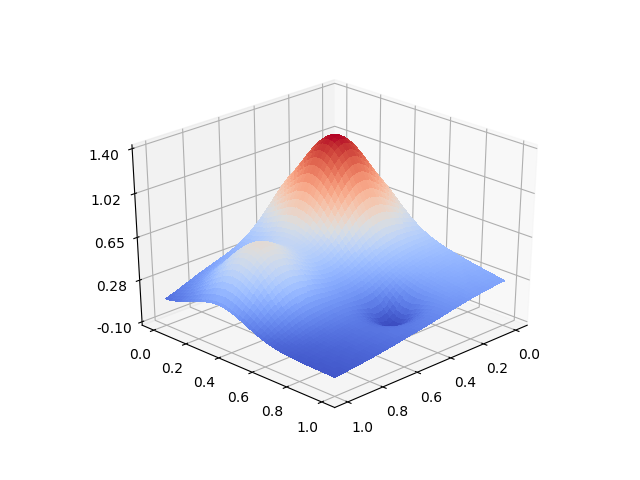
\includegraphics[width=\linewidth]{franke.png}
\captionof{figure}{The Franke test function plotted for $0\le x,y\le 1$. \label{fig:1}}
\end{Figure}

\subsection{Terrain data}
The terrain data used is taken from the U.S. Department of the Interior U.S. Geological Survey's (USGS) EarthExplorer\footnote{EarthExplorer website: \url{https://earthexplorer.usgs.gov/}.} website. The USGS stores data from the Shuttle Radar Topography Mission (SRTM) which maps the earth's land surface topology with a resolution of 1 arc-second (about $30\,\text{m}$). We will use SRTM data taken from the EarthExplorer website as the basis for our terrain parametrization.

The specific terrain data we will use in the present project is taken from the Møsvatn Austfjell area in the municipality of Tinn in Telemark county, Norway. A visual representation of the data is shown in \fig{2}. 

\begin{Figure}
\centering

\includegraphics[width=\linewidth]{terrain2.png}
\captionof{figure}{The terrain data in use in the present work, taken from the Møsvatn Austfjell area in the municipality of Tinn in Telemark county, Norway. Retrieved using the USGS EarthExplorer website. The height data is scaled to fit in $0\le z\le 1$, and the reference zero point is set to zero. \label{fig:2}}
\end{Figure}


\section{Results and discussion}
\subsection{Verification of the models: The Franke function}

\newlength{\myrowskip}
\setlength{\myrowskip}{10pt}
\begin{table*}
\centering\sisetup{table-number-alignment=center}
\setlength\extrarowheight{2pt}
\begin{tabularx}{\textwidth}{X*{9}{S[table-format=-2.3]}}
\toprule
$p$       & \multicolumn{2}{>{\hsize=\dimexpr2\hsize}c}{$2$}                         & \multicolumn{2}{>{\hsize=\dimexpr2\hsize}c}{$3$}                        & \multicolumn{2}{>{\hsize=\dimexpr2\hsize}c}{$4$}                            & \multicolumn{2}{>{\hsize=\dimexpr2\hsize}c}{$5$}                             \\
          & \multicolumn{1}{>{\hsize=\dimexpr1\hsize}c}{$\beta$} & \multicolumn{1}{>{\hsize=\dimexpr1\hsize}c}{$\sigma^2(\beta)$}   & \multicolumn{1}{>{\hsize=\dimexpr1\hsize}c}{$\sigma^2(\beta)$} & \multicolumn{1}{>{\hsize=\dimexpr1\hsize}c}{$\beta$} & \multicolumn{1}{>{\hsize=\dimexpr1\hsize}c}{$\sigma^2(\beta)$}& \multicolumn{1}{>{\hsize=\dimexpr1\hsize}c}{$\beta$} & \multicolumn{1}{>{\hsize=\dimexpr1\hsize}c}{$\sigma^2(\beta)$}& \multicolumn{1}{>{\hsize=\dimexpr1\hsize}c}{$\beta$} &  \\
\midrule
$1$       &  1.17606 & 0.00007 &  0.99432 & 0.00014 &   0.60714 & 0.00006 &   0.37920 & 0.00052 \\[\myrowskip]
$x$       & -1.06533 & 0.00047 & -0.60390 & 0.00314 &   4.23195 & 0.00478 &   8.05787 & 0.03989 \\
$y$       & -0.74196 & 0.00041 &  1.36710 & 0.00206 &   3.18895 & 0.00399 &   3.77385 & 0.03382 \\[\myrowskip]
$x^2$     &  0.12032 & 0.00026 & -1.40195 & 0.00885 & -19.38216 & 0.05541 & -35.01195 & 0.52045 \\
$xy$      &  0.87501 & 0.00025 &  2.04306 & 0.00597 &  -2.28349 & 0.02825 & -15.64235 & 0.50091 \\
$y^2$     & -0.36720 & 0.00029 & -6.65928 & 0.00585 & -12.53672 & 0.04434 &  -8.30869 & 0.44047 \\[\myrowskip]
$x^3$     &          &         &  0.89177 & 0.00288 &  25.25628 & 0.10794 &  49.21854 & 1.61746 \\
$x^2y$    &          &         &  0.36261 & 0.00219 &   8.10444 & 0.05690 &  45.87508 & 1.70397 \\
$xy^2$    &          &         & -1.50662 & 0.00188 &   1.40554 & 0.05242 &  21.25127 & 1.47419 \\
$y^3$     &          &         &  4.69644 & 0.00207 &  12.61520 & 0.08471 &  -9.03064 & 1.50607 \\[\myrowskip]
$x^4$     &          &         &          &         & -10.84136 & 0.02548 & -24.13509 & 1.25784 \\
$x^3y$    &          &         &          &         &  -5.15114 & 0.01948 & -54.81283 & 1.39124 \\
$x^2y^2$  &          &         &          &         &   0.00764 & 0.01437 &  -8.23581 & 1.14134 \\
$xy^3$    &          &         &          &         &  -1.90524 & 0.02013 & -30.19186 & 1.12319 \\
$y^4$     &          &         &          &         &  -3.51179 & 0.02032 &  30.20166 & 1.28260 \\[\myrowskip]
$x^5$     &          &         &          &         &           &         &   1.53882 & 0.16041 \\
$x^4y$    &          &         &          &         &           &         &  19.53504 & 0.18567 \\
$x^3y^2$  &          &         &          &         &           &         &  10.83952 & 0.17047 \\
$x^2y^3$  &          &         &          &         &           &         &  -5.29938 & 0.15935 \\
$xy^4$    &          &         &          &         &           &         &  16.91243 & 0.15035 \\
$y^5$     &          &         &          &         &           &         & -16.84369 & 0.16920 \\
\bottomrule 
\end{tabularx}
\caption{Parameters $\beta$ and their bootstrap computed variance $\sigma^2(\beta)$ for the OLS fits of the Franke function, shown in \fig{3}. \label{tab:1}}
\end{table*}



\begin{figure*}[p]
\vspace{-50pt}
\centering
\subfloat[$p=2$]{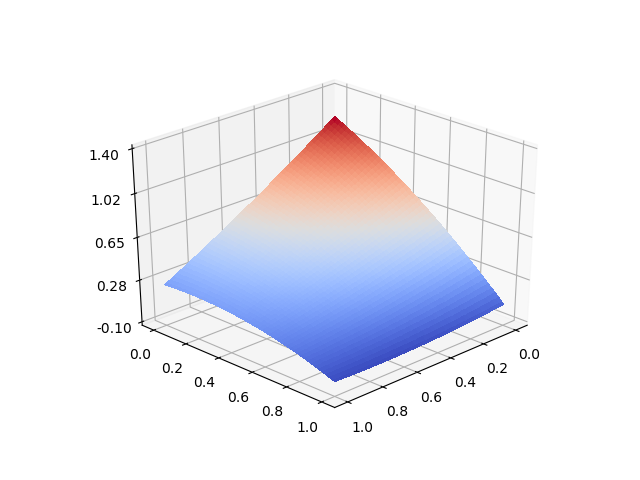
\includegraphics[width=0.4\linewidth]{OLS2.png}}
\subfloat[$p=3$]{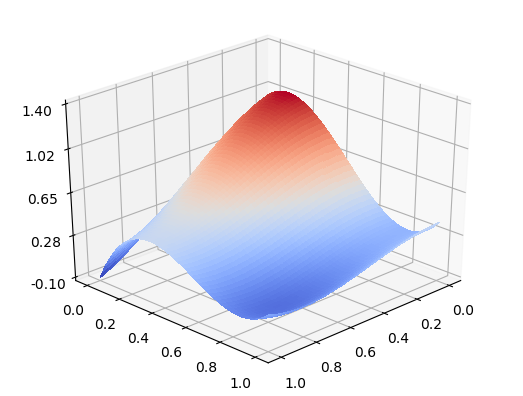
\includegraphics[width=0.4\linewidth]{OLS3.png}} \\[-20pt]
\subfloat[$p=4$]{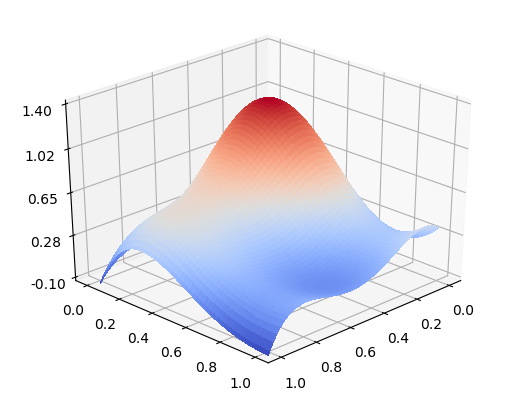
\includegraphics[width=0.4\linewidth]{OLS4.png}}
\subfloat[$p=5$]{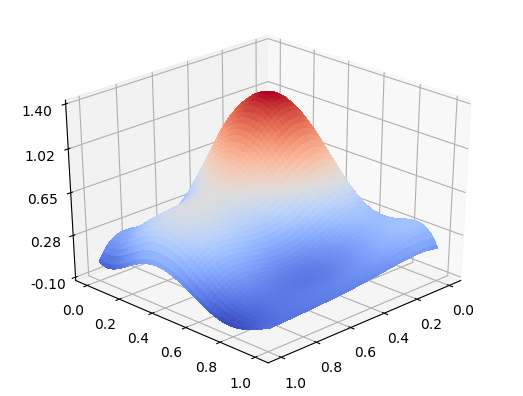
\includegraphics[width=0.4\linewidth]{OLS5.png}}
\captionof{figure}{Ordinary least squares fits, using data from the Franke function with polynomials of degree $2$, $3$, $4$, and $5$. The $p$ parameter indicates what order of polynomials are used. The target function of Franke can be seen in \fig{1}. \label{fig:3}}
\end{figure*}
\begin{figure*}[p]
\centering
\subfloat[$p=2$]{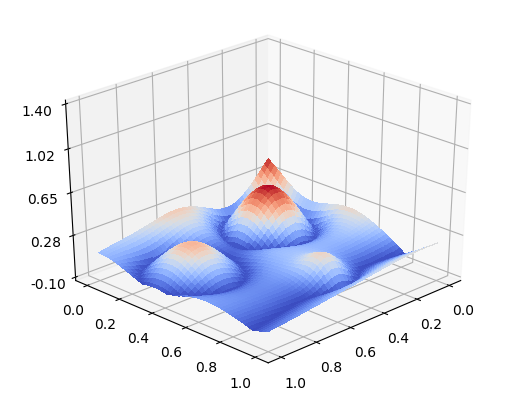
\includegraphics[width=0.4\linewidth]{OLS2_diff.png}}
\subfloat[$p=3$]{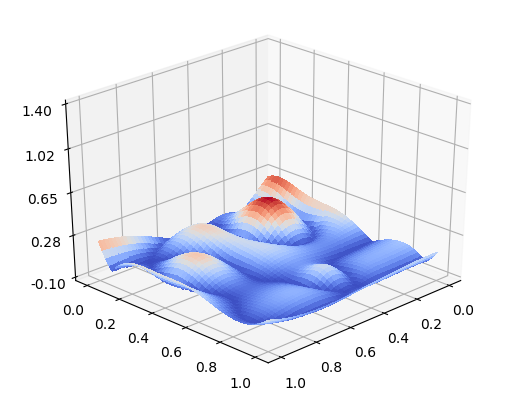
\includegraphics[width=0.4\linewidth]{OLS3_diff.png}} \\[-20pt]
\subfloat[$p=4$]{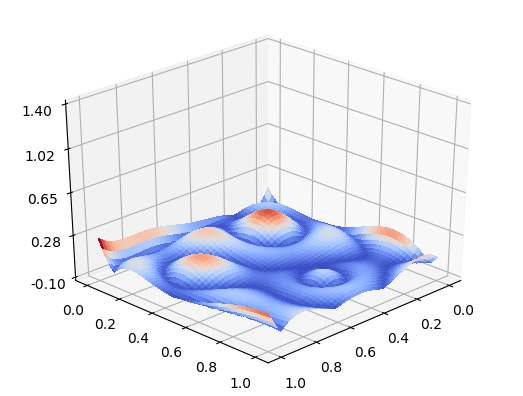
\includegraphics[width=0.4\linewidth]{OLS4_diff.png}}
\subfloat[$p=5$]{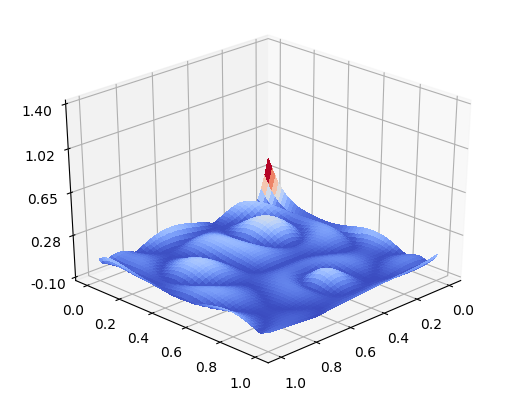
\includegraphics[width=0.4\linewidth]{OLS5_diff.png}}
\captionof{figure}{The absolute difference between the ordinary least squares fits of \fig{3} and the true data, the Franke function. Polynomials of degree $2$, $3$, $4$, and $5$ have been used in the fitting. The $p$ parameter indicates what order of polynomials are used. \label{fig:4}}
\end{figure*}


\subsection{Terrain data parametrization}
\lipsum[3]

\section{Conclusion}
\lipsum[3]
\end{multicols}


\printbibliography[heading=bibintoc]
\end{document}



